\documentclass[a4paper]{article}

\usepackage[brazilian]{babel}
\usepackage[utf8x]{inputenc}
\usepackage[T1]{fontenc}

\usepackage{listings}

%% Useful packages
\usepackage{amsmath}
\usepackage{graphicx}
\usepackage[colorinlistoftodos]{todonotes}
\usepackage[colorlinks=true, allcolors=blue]{hyperref}

\usepackage{mathrsfs}
\usepackage{amssymb}



%opening
\title{Relatório do exercício prático II (E2)}
\author{Daniel Moreira Cestari - 5746193}

\begin{document}

\maketitle

%\section{Introdução}

% execuções 
% repel => python poisson.py airfoil.txt saida.vtk 100 '' '' '0.5,0.5' '' '-5' '' '20' '' '-5' '' '20'
% atract => python poisson.py airfoil.txt saida.vtk 100 '' '' '0.5,0.5' '' '20' '' '20' '' '20' '' '20'
% border refinement 1 => python poisson.py airfoil.txt saida.vtk 100 '0.45' '1.0' '0.5,0.5' '5' '5' '5' '5' '5' '5' '5' '5'
% border refinement 2 => python poisson.py airfoil.txt saida.vtk 100 '0.45' '1.0' '0.45,1.0' '5' '5' '5' '5' '20' '5' '20' '5'

Este trabalho visa a utilização do método TTM baseado nas equações de Poisson para refinamento de malhas geradas automaticamente.

Como explicado no final do exercício 1, o uso de funções de controle para refinar a malha em regiões de interesse podem corrigir alguns problemas que ocorrem com a geração automática utilizando a equação de Laplace.

Essas regiões de interesse podem ser especificadas como retas nos eixos computacionais, $\xi_i$ e $\eta_j$, ou pontos especificados também no domínio computacional, $(\xi_k,\eta_k)$.

O código passado em aula novamente foi convertido do formato do \textit{jupyter notebook} para \textit{python} e modificados. As modificações foram a adição do resto do método TTM, em sala foi implementado parcialmente, apenas permitindo o refinamento em $\xi$. Foram, então, adicionados os refinamentos para $\eta$ e para pontos específicos. Também permite agora incluir mais de um eixo para $\xi_i$, $\eta_i$ e mais de um ponto, e também é possível escolher um parâmetro específico para cada ponto de controle. Por exemplo, pode-se aproximar reta de uma $\xi_i$ e repelir de outra $\xi_j$. Esta última figura está diferente das anteriores porque seu tamanho é maior, mas um \textit{zoom} na mesma permite sua perfeita visualização.

Todos os parâmetros necessários são passados por linha de comando seguindo o seguinte padrão:

\begin{verbatim}
python poisson.py filename.txt save_file.vtk iter_number 
xis_rf etas_rf points_rf 
a_xis b_xis c_xis d_xis 
a_etas b_etas c_etas d_etas
\end{verbatim}

O primeiro parâmetro, \textit{filename}, é o arquivo com a definição dos bordos, \textit{save\_file.vtk} especifica o nome do arquivo \textit{vtk} gerado, \textit{iter\_number} refere-se ao número de iterações do método. Os parâmetros \textit{xis\_rf}, \textit{etas\_rf} e \textit{points\_rf}, são listas contendo os pontos de controle, \textit{xis\_rf} e \textit{etas\_rf} são separados por vírgula, já \textit{points\_rf} tem duas coordenadas para cada ponto, as coordenadas são separadas por vírgula e os pontos são separados com ponto-e-vírgula. Os pontos de controle como estão especificados no domínio computacional estão limitados no intervalo $[0,1]$. Os outros 8 parâmetros são listas para os parâmetros do método TTM, $a$, $b$, $c$ e $d$, para cada ponto de controle, $\xi_i$ e $\eta_j$ e pontos.

Abaixo é fornecido um exemplo de execução:

\begin{verbatim}
python poisson.py swan.txt saida.vtk 100 
'0.1' '0.1' '' 
'5' '5' '5' '5' 
'5' '5' '5' '5'
\end{verbatim}

A quebra de linha foi adicionada apenas para melhorar a visualização, e as aspas foram adicionadas para permitir a passagem de argumentos vazios. Esse exemplo é o da Figura \ref{fig:swan}, que atrai as linhas $\xi$ para a coordenada $0.1$ e $\eta$ também para a coordenada $0.1$. Na figura é possível ver que o problema que ocorreu no exercício prático 1 de pontos fora do domínio não ocorre com o uso de pontos de controle.

As Figuras \ref{fig:airfoil_attract_point} e \ref{fig:airfoil_repel_point} foram geradas experimentando os parâmetros do método de controle. Na primeira é feita uma atração para o ponto $(0.5,0.5)$, enquanto que na segunda foi feita uma repulsão no mesmo ponto. Percebeu-se uma menor sensibilidade dos parâmetros \textit{b} e \textit{d} para a atração. Nesses exemplos, foi utilizado $b=d=20$ para atração e $b=d=-5$ para repulsão. Na descrição das figuras é apresentado o código para geração da mesma.

Por fim, na Figura \ref{fig:airfoil_refinement} é apresentada o refinamento da malha ao redor do aerofólio e na parte frontal do mesmo. Os parâmetros utilizados foram $\xi=0.45$ para pegar as linhas incidentes ao perfil na parte frontal, $\eta=1.0$ para pegar as linhas ao redor do perfil, e o ponto $(0.45,1.0)$ para refinar mais exatamente na parte frontal do perfil. Para essa execução pode-se chamar o código sem passar nenhum parâmetro que os valores \textit{default} estão configurados para esse caso. 

% execuções 
% repel => python poisson.py airfoil.txt saida.vtk 100 '' '' '0.5,0.5' '' '-5' '' '20' '' '-5' '' '20'
% atract => python poisson.py airfoil.txt saida.vtk 100 '' '' '0.5,0.5' '' '20' '' '20' '' '20' '' '20'
% border refinement 1 => python poisson.py airfoil.txt saida.vtk 100 '0.45' '1.0' '0.5,0.5' '5' '5' '5' '5' '5' '5' '5' '5'
% border refinement 2 => python poisson.py airfoil.txt saida.vtk 100 '0.45' '1.0' '0.45,1.0' '5' '5' '5' '5' '20' '5' '20' '5'


\begin{figure}[ht]
	\centering
	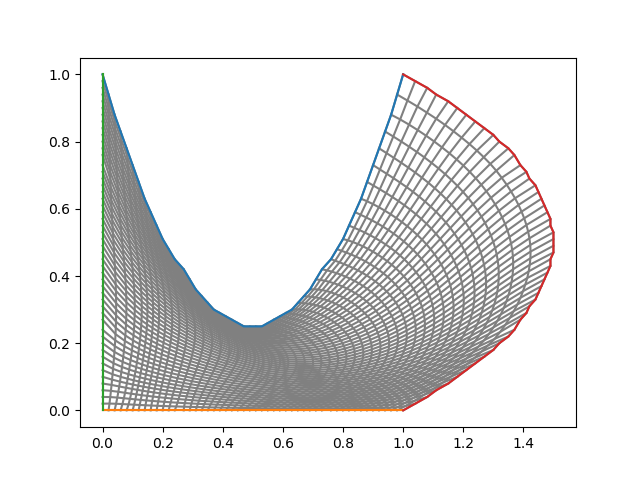
\includegraphics[width=1.0\textwidth]{swan_0,1_0,1.png}
	\label{fig:swan} 
	\caption[caption]{Curva \textit{swan} com pontos de controle $\xi=0.1$ e $\eta=0.1$. \\\hspace{\textwidth} \textit{python poisson.py swan.txt saida.vtk 100 '0.1' '0.1' '' '5' '5' '5' '5' '5' '5' '5' '5'}}
\end{figure}


\begin{figure}[ht]
	\centering
	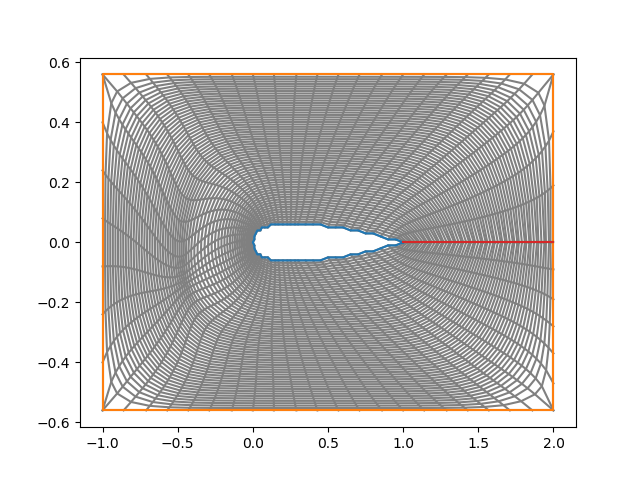
\includegraphics[width=1.0\textwidth]{airfoil_attract_point.png}
	\label{fig:airfoil_attract_point} 
	\caption[caption]{Testando atração de ponto de controle na curva \textit{airfoil}. \\\hspace{\textwidth} \textit{python poisson.py airfoil.txt saida.vtk 100 '' '' '0.5,0.5' '' '20' '' '20' '' '20' '' '20'}}
\end{figure}



\begin{figure}[]
	\centering
	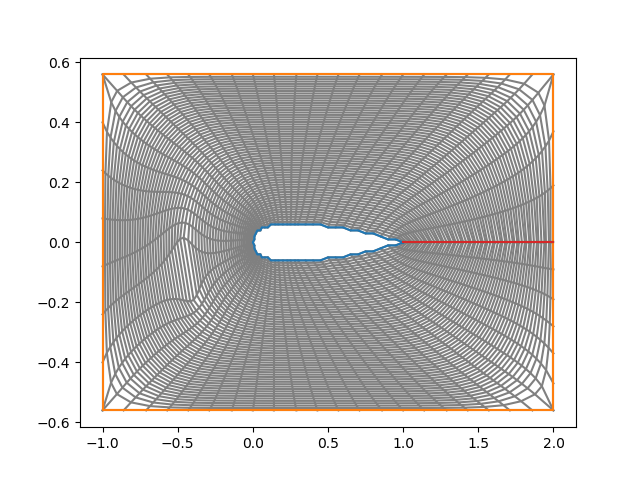
\includegraphics[width=1.0\textwidth]{airfoil_repel_point.png}
	\label{fig:airfoil_repel_point} 
	\caption[caption]{Testando repulsão de ponto de controle na curva \\textit{airfoil} . \\\hspace{\textwidth} \textit{python poisson.py airfoil.txt saida.vtk 100 '' '' '0.5,0.5' '' '-5' '' '20' '' '-5' '' '20'}}
\end{figure}


\begin{figure}[ht]
	\centering
	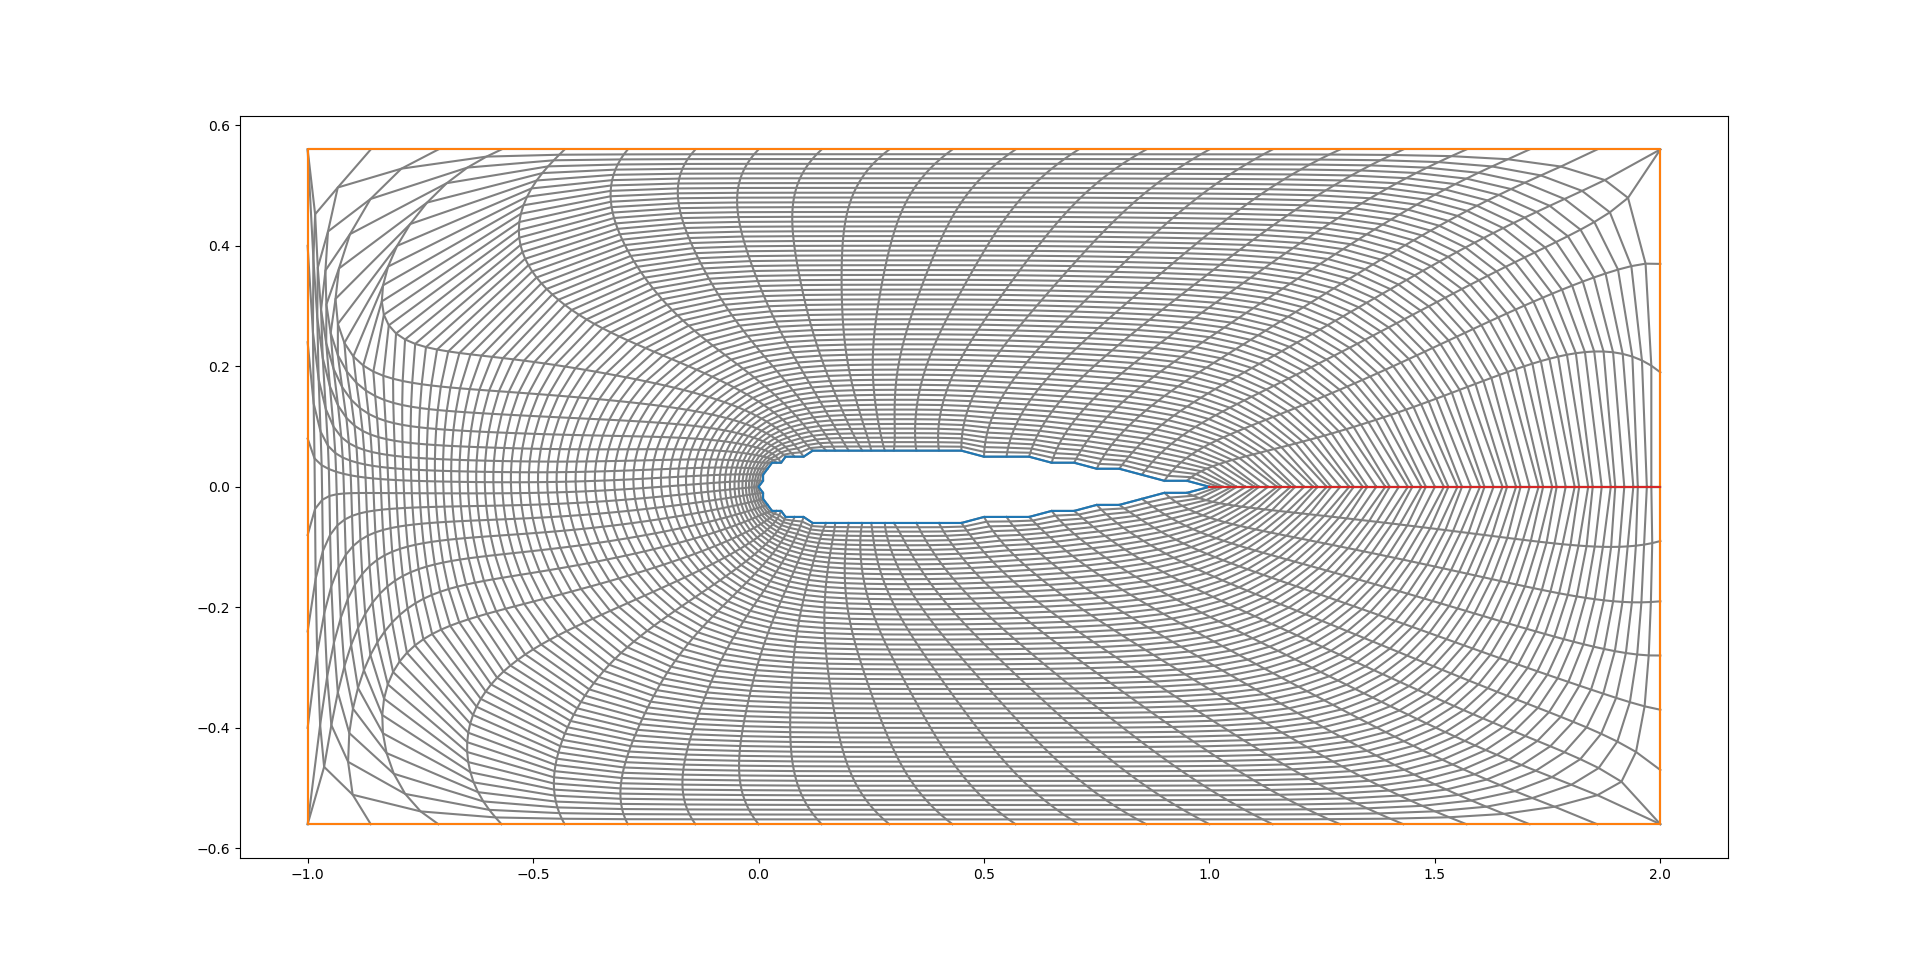
\includegraphics[width=1.0\textwidth]{airfoil_border_refinement6.png}
	\label{fig:airfoil_refinement} 
	\caption[caption]{Refinamento da malha para o perfil da curva \textit{airfoil} utilizando pontos de controle. \\\hspace{\textwidth} \textit{python poisson.py airfoil.txt saida.vtk 100 '0.45' '1.0' '0.45,1.0' '5' '5' '5' '5' '5' '5' '5' '5'}}
\end{figure}


Com esse exercício prático foi possível verificar que a utilização de pontos de controle permite melhorar a geração automática de malhas. Também verificou-se que os valores dos parâmetros do método TTM têm de ser definidos e não há uma heurística para a definição desses valores, é preciso experimentar.


\end{document}
